% This text is proprietary.
% It's a part of presentation made by myself.
% It may not used commercial.
% The noncommercial use such as private and study is free
% Sep. 2005 
% Author: Sascha Frank 
% University Freiburg 
% www.informatik.uni-freiburg.de/~frank/
%
% additional usepackage{beamerthemeshadow} is used
\documentclass{beamer}
\usepackage{beamerthemeshadow}
\usepackage[utf8]{inputenc} % set input encoding (not needed with XeLaTeX)
\usepackage[T1]{fontenc}

\begin{document}
\title{Web Media Manager}  
\author{Jean-Philippe Froelicher}
\date{\today} 

\frame{\titlepage} 

\frame{\frametitle{Sommaire}\tableofcontents[hideallsubsections]} 


\section{Introduction} 
\subsection{Sujet}
\frame{\frametitle{Sujet} 
\begin{itemize}
	\item Projet de diplôme
	\item Réalisation d'une application
	\item Application évolutive et souple
	\item Utilisation des API REST
\end{itemize}
}

\subsection{Glossaire}
\frame{\frametitle{Glossaire} 
	Each frame should have a title.
}

\subsection{Média vidéo du Web}
\frame{\frametitle{Média vidéo du Web} 
	\begin{itemize}
		\item Plate-forme d'hébergement vidéo.
		\item Twitch ; Youtube ; Dailymotion ; Vimeo ; Ustream etc.
		\item Vidéo à la demande (VOD) ; Diffusion de flux vidéo. en direct.
		\item Rémunération suivant le nombres de vues ; Dons.
	\end{itemize}
}



\section{Principales fonctionnalités} 
\subsection{Fonctions de bases}
\frame{\frametitle{Fonctions communes} 
	\begin{itemize}
		\item Connexion à un compte
		\item Visionnage d'une vidéo / vidéo en direct
		\item S'abonner à une chaîne
		\item Chat IRC pour les vidéos en direct
		\item Recherche de vidéos
		\item Vidéos actuellement en direct ; Dernières vidéos
		\item Chaînes abonnées
	\end{itemize}
}
\subsection{Notifications}
\frame{\frametitle{Notifications} 
	Lorsqu'une nouvelle diffusion en direct commence ou qu'une vidéo sort.
	\begin{itemize}
		\item Pop-up qui apparaît avec les informations de la vidéo.
	\end{itemize}
	Les notifications servent à être mis au courant le plus rapidement possible.
}
\subsection{Chat IRC}
\frame{\frametitle{Chat IRC} 
	Internet Relay Chat, Protocole de communication textuelle.
	Uniquement sur les vidéos en direct.
	\begin{figure}[h]
		\center
		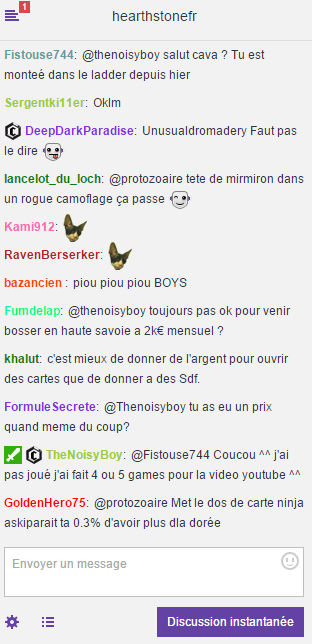
\includegraphics[width=0.2\textwidth]{chatIrc.png}
		\caption{Chat Irc}
	\end{figure}
	
}
\subsection{Catégorie \& Liste de lectures}
\frame{\frametitle{Catégorie \& Liste de lectures} 
	Les catégories servent à rassembler un certain nombre de vidéos de sites différents.
	
	Les listes de lectures servent à lire à la suite les vidéos quelle contient.
}


\section{Mise en oeuvre}

\subsection{Conception}
\frame{\frametitle{Conception} 
	Site générique \\
	Classe de base
	\begin{figure}[h]
		\center
		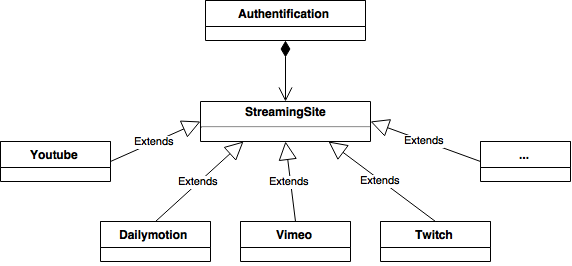
\includegraphics[width=0.7\textwidth]{StreamingSite.png}
		\caption{Diagramme}
	\end{figure}
}

\subsection{SVideo \& SChannel}
\frame{\frametitle{SVideo \& SChannel} 
	Structures rassemblant les informations communes de toutes les vidéos et chaînes des différents sites.\\
	Toutes les vidéos et les chaînes de l'application sont transtypés en cette structure ainsi je peux faire tout les traitements de la même manière.
	
	\begin{figure}[h]
		\center
		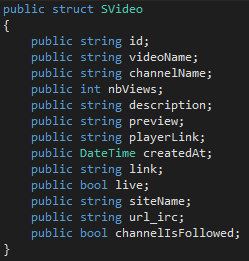
\includegraphics[width=0.25\textwidth]{SVideo.png}
		\caption{Commande cURL}
	\end{figure}
	
}

\subsection{Récupération des données}
\frame{\frametitle{Récupération des données} 
	API des différents sites.
	Données reçuent en JSON 
	
	Librarie cURL utilisé : GET, POST, PUT, DELETE
	
	\begin{figure}[h]
		\center
		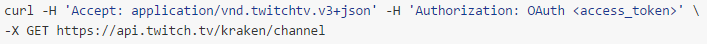
\includegraphics[width=1\textwidth]{curl.png}
		\caption{Commande cURL}
	\end{figure}
}

\frame{\frametitle{Classes structures} 
	Afin de reçevoir les données dans un bon type, il faut créer les classes structures pour chaque sites.
	
	\begin{figure}[h]
		\center
		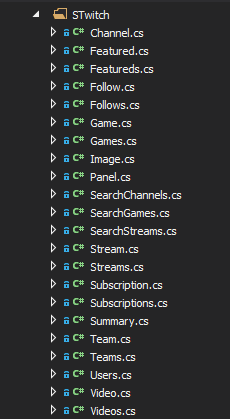
\includegraphics[width=0.2\textwidth]{STwitch.png}
		\caption{Classes Twitch}
	\end{figure}
}

\frame{\frametitle{Désérialisation} 
	Type générique et lors de lappel de la methode on indique une classe structure.
	\begin{figure}[h]
		\center
		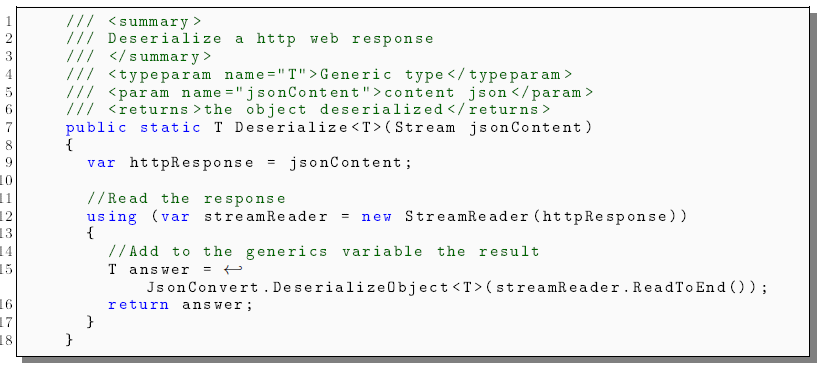
\includegraphics[width=0.7\textwidth]{deserialize.png}
		\caption{Classes Twitch}
	\end{figure}
}

\subsection{Connexion}
\frame{\frametitle{Connexion} 
	Connexion grâce au protocole OAuth2.\\
	Utilisation du lien API de connexion.\\
	Récupération du jeton d'accès dans l'url.
	\begin{itemize}
		\item Création d'un GitHub Page
	\end{itemize}
}

\subsection{Notifications}
\frame{\frametitle{Notifications} 
	Vérification toutes les 5 secondes
	\begin{itemize}
		\item Comparaison de deux listes
		\item Multi-Thread
	\end{itemize}
	
	Composant venant du Web
	\begin{itemize}
		\item NotificationWindow
	\end{itemize}
	
	\begin{figure}[h]
		\center
		
\includegraphics[width=0.7\textwidth]{notificationview.png}
		\caption{Exemple d'une notification}
	\end{figure}
}

\subsection{Catégorie \& liste de lectures}
\frame{\frametitle{Catégorie \& Liste de lectures} 
	Stockage dans un fichier de type INI dans le dossier appdata de l'utilisateur.
	
	Les vidéos sont stockés sous forme de liens.
	\begin{figure}[h]
		\center
		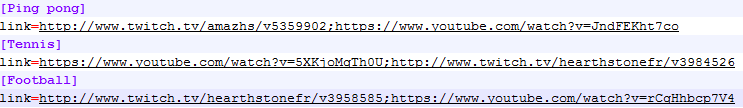
\includegraphics[width=0.7\textwidth]{inifile.png}
		\caption{Exemple du fichier INI}
	\end{figure}
	
	
}

\section{Conclusion \& perspectives}
\subsection{Conclusions}
\frame{\frametitle{Conclusions} 
	Conclusion technique : 
	\begin{itemize}
		\item Application fonctionnelle
		\item Cahier des charges pas remplit
	\end{itemize}
	
	Conclusion personnelle :
	\begin{itemize}
		\item Plaisant de travailler sur un gros projet
	\end{itemize}	
}

\section{Démonstration} 
\frame{\frametitle{Démonstration} 
}
	
\section{Questions} 
\frame{\frametitle{Questions} 
}
\end{document}

